\section{Evaluación y resultados}

%En esta sección se explicarán las metodologías utilizadas para 
%evaluar la solución y los principales resultados obtenidos.

En la tabla~\ref{tab:metodologia} se observan las metodologías utilizadas
para la evaluación de la solución incluyendo la determinación de la muestra.

\begin{table}[H]
\centering
\begin{tabulary}{.5\textwidth}{rLLLL}
\toprule
\textbf{Prueba}        & \textbf{Determinar la muestra} & \textbf{Evaluar el uso y la aceptación de la solución} & \textbf{Evaluar el conocimiento de los alumnos} \\
\midrule
\textbf{Participantes} & \multicolumn{3}{c}{Alumnos de la carrera de enfermería del IAB} \\
\midrule
\textbf{Muestra}       & 124 Alumnos                                                        & 11 Alumnos                     & 124 alumnos \\
\midrule
\textbf{Lugar}         & IAB                                                                &                                & IAB\\
\midrule
\textbf{Duración}      & 10 minutos                                                         & 20 días                        & 20 minutos\\
\midrule
\textbf{Fases}           & \tabitem Presentación.          & \tabitem Explicación de la interfaz. & \tabitem Explicación de la prueba.\\
                & \tabitem Encuesta.              & \tabitem Utilización de la solución. & \tabitem Encuesta sobre conocimiento\\
                & \tabitem Recopilación de datos. & \tabitem Encuesta de apreciación.    & \tabitem Recopilación de datos.\\
                &                                 & \tabitem Recopilación de datos.\\
\bottomrule
\end{tabulary}
\label{tab:metodologia}
\end{table}

A continuación se describen los detalles de la metodologías utilizadas junto con
los principales resultados obtenidos.

%Comentarios de tincho:
% A quien se le hizo el test (muestra)
% Correlación
% Resumen de todo
% Encuesta objetiva
% Explicar a quien se le hizo el test, resumen, correlación
%3 paginas

\subsection{Encuesta para determinar la muestra}
\label{encuesta_muestra}

Con esta encuesta se determinó el nivel de
acceso a la tecnología de los estudiantes del cuarto año de Licenciatura en
Enfermería del \gls{iab}, además del tipo de acceso a Internet, tipo de sistema
operativo de sus teléfonos móviles y si cumplían con los requisitos técnicos
para utilizar la solución. Estos requisitos son los siguientes:  memoria RAM de
$512$MB. o superior, velocidad de procesador de $800$ GHz. o superior y GPU Mali
400 o superior. 

A continuación se muestran los resultados.

\begin{figure}[H]
\centering
\begin{tikzpicture}[thick,scale=0.7, every node/.style={transform shape}]
    \pie[
        text=legend,
        explode=.1,
        style=drop shadow,
        ]%
    {%
        81.7 / No cumple,
        18.3 /  Cumple
    }
\end{tikzpicture}
\caption{Dispositivos que cumplen con los requisitos mínimos para la prueba}
\label{fig:ubicacion_requisitos_minimos}
% TODO se debe ver los requisitos en esta misma página.
\end{figure}

\begin{figure}
\centering
\begin{tikzpicture}[thick,scale=0.7, every node/.style={transform shape}]
    \pie[
        %explode=.2,
        text=legend,
        style=drop shadow,
        %radius=3,
        %scale font,
        explode={0.1,0.1,0.3,0.3}
        ]%
    {%
        31.2 / Plan pos-pago,
        57   / Paquetes pre-pago,
        5.4  / Sin acceso,
        6.4  / Acceso ocasional}
\end{tikzpicture}
\caption{Acceso a internet desde dispositivos móviles}
\label{fig:ubicacion_acceso_internet}
\end{figure}

\begin{figure}
\centering
\begin{tikzpicture}[thick,scale=0.7, every node/.style={transform shape}]
    \pie[
        text=legend,
        rotate=61.3,
        explode={.1,.2,.2,.2},
        style=drop shadow,
        ]%
    {%
    61.3 / Android,
     8.6 / Symbian,
    12.9 / Windows Phone,
    17.2 / Otros}
\end{tikzpicture}
\caption{Sistemas operativos móviles utilizados}
\label{fig:ubicacion_sistemas_operativos}
\end{figure}


Del $18.3\%$ de los que cumplían con los requisitos, $11$ alumnos estuvieron
dispuestos a evaluar la solución. 

El estudio~\cite{nielsen2000} establece que la cantidad de usuarios requeridos
para las pruebas de \gls{gui} dependen del nivel de experiencia de los usuarios
con tecnología similar, y~\cite{ritch2009} define el rango de usuarios
necesarios para resultados estadísticamente válidos, cuando los mismos no tienen experiencia con la tecnología, de $10$ a $12$.
% La muestra utilizada en las pruebas de la solución es de $11$ usuarios.

\subsection{Encuesta para evaluar la solución}
\label{encuesta_solucion}
Con esta encuesta se busca identificar las fortalezas y debilidades de la 
solución, además de evaluar la solución en cuanto a factores de exploración, 
representación, motivación, inmersión, retroalimentación y pedagogía. También se busca valorar el nivel de aceptación de la solución y la validación de las 
hipótesis planteadas como parte del diseño de la solución.

La encuesta cuenta con $27$ preguntas cerradas, es decir de una sola respuesta 
en una lista de opciones, y con $4$ preguntas abiertas, es decir los encuestados pueden dar respuestas libres a las preguntas. 

En las preguntas cerradas la métrica utilizada es la escala de Likert
\cite{Allen:2007} de 7 valores posibles cuyo valor más alto es
\enquote{Totalmente de acuerdo} y el más bajo es \enquote{Totalmente en 
desacuerdo}. 

Una vez valoradas y registradas todas las respuestas y con el 
objetivo de eliminar las tendencias en la forma en la que son completadas las
encuestas\cite{Fischer2010} se utiliza el método de \emph{Doble 
Estandarización} recomendado en~\cite{Pagolu2011}, el promedio estandarizado 
refleja los puntos fuertes y débiles relativos a la valoración más alta y baja.

En el cuadro~\ref{tab:resultado_resumen_aspectos_aceptacion} se observa 
la aceptación de los usuarios por aspecto estudiando. El 
cuadro~\ref{tab:resultado_resumen_hipotesis} se observa la aceptación
de los usuarios por hipótesis asumida.  

\begin{table}
\centering
\caption{Aceptación por aspecto de la solución}
\begin{tabular}{lcr}
\toprule
Factores        & Promedio encuesta      & Promedio estandarizado \\
\midrule
Motivación               & De acuerdo              & $0.67$  \\
Facilidad de exploración & De acuerdo              & $0.68$  \\
Sensación de Inmersión   & De acuerdo              & $0.63$  \\
Pedagogía                & De acuerdo              & $0.67$  \\
Representación           & Parcialmente de acuerdo & $0.53$  \\
Retroalimentación        & Parcialmente de acuerdo & $0.60$  \\
Utilidad                 & De acuerdo              & $0.69$  \\
\bottomrule
\end{tabular}
\label{tab:resultado_resumen_aspectos_aceptacion}
\end{table}



\begin{table}
\centering
\caption{Hipótesis con su aceptación}
\begin{tabular}{lcr}
\toprule
Hipótesis                   & Promedio encuesta     & Promedio estandarizado \\
\midrule
H1. Comandos de voz         & De acuerdo              & $0,55$ \\
H2. Extracción de elementos & Parcialmente de acuerdo & $0,65$ \\
H3. Bioseguridad            & De acuerdo              & $0,58$ \\
H4. Iconos                  & Parcialmente de acuerdo & $0,53$ \\
H5. Motivación              & De acuerdo              & $0,65$ \\
H6. Retroalimentación       & De acuerdo              & $0,61$ \\
H7. Ubicuidad               & De acuerdo              & $0,66$ \\
\bottomrule
\end{tabular}
\label{tab:resultado_resumen_hipotesis}
\end{table}



\begin{figure}
\centering
\begin{tikzpicture}[label distance=.15cm]
\tkzKiviatDiagram[scale=.5,%
                    lattice=9,
                    %step=10,
                    ]
                {Motivación,
                 Exploración,
                 Inmersión,
                 Pedagogía,
                 Representación,
                 Retroalimentación,
                 Utilidad}
\tkzKiviatLine[thick,
                color=blue!25!white,
                mark=ball,
                ball color=blue,
                mark size=5pt,
                opacity=.2, 
                fill=blue!20](6.7,6.8,6.3,6.7,5.3,6.0,6.9)
\tkzKiviatGrad[prefix={$0,$}](1) 
\end{tikzpicture}
\label{fig:subjetiva_kiviat}
\caption{Gráfico de Kiviat de los factores evaluados}
\end{figure}

\subsection{Encuesta para evaluar el conocimiento}

Esta encuesta mide el nivel de conocimiento de los alumnos sobre los dos temas 
simulados, contiene preguntas de nivel básico, medio y avanzado. Las mismas 
son formuladas utilizando la lista de competencias básicas que debe tener un 
alumno para aprobar la materia \textbf{Enfermería en Urgencias II}. Las 
preguntas son validadas  por los profesores de la cátedra. Cada pregunta 
tiene el mismo peso, así la puntuación más baja obtenible es $0$, y la más 
alta es $10$. La encuesta fue aplicada a la muestra y a un grupo de control 
compuesto por los demás estudiantes de la población objetivo.

De esta manera se busca evaluar la influencia pedagógica  de la solución en el
aprendizaje. Dado que la cantidad de partidas jugadas por usuario por tipo de
procedimiento no es considerada suficiente no se pueden considerar las
diferencias entre la muestra y el grupo de control como absolutas. En el
cuadro~\ref{tab:objetiva_rendimiento_por_pregunta} se observan los resultados de esta prueba.

\begin{table}
\centering
\caption{Rendimiento promedio de usuarios por pregunta}
\begin{tabular}{lrrr}
\toprule
& \multicolumn{3}{c}{Promedio} \\
\cmidrule(lr){2-4}
\textbf{Pregunta} & 
\textbf{Muestra} & 
\textbf{Grupo Control} & 
\textbf{Total} \\ 
\midrule
ES1. Torniquete           & 0.36 & 0.18 & 0.20 \\
ES2. Guantes              & 0.64 & 0.60 & 0.60 \\
ES3. Manos                & 0.09 & 0.14 & 0.13 \\
ES4. Bioseguridad         & 0.27 & 0.25 & 0.26 \\
ES5. Explicación          & 0.82 & 0.56 & 0.59 \\
\midrule
EG1. Diagnóstico Global 1 & 0.00 & 0.18 & 0.16 \\
EG2. Diagnóstico Global 2 & 0.64 & 0.51 & 0.53 \\
EG3. Respuesta ocular     & 0.45 & 0.28 & 0.29 \\
EG4. Respuesta motora     & 0.18 & 0.32 & 0.31 \\
EG5. Respuesta verbal     & 0.36 & 0.45 & 0.45 \\
\midrule
\textbf{Promedio}: & 3.82 & 3.47 & 3.49  \\
\bottomrule
\end{tabular}

\label{tab:objetiva_rendimiento_por_pregunta}
\end{table}

\subsection{Registro de actividades}

La solución propuesta almacena información relacionada a la actividad del
usuario, incluyendo cuando y como utiliza las acciones, los pasos que realiza,
el orden y las condiciones de la escena cuando realiza cada acción, el tiempo de partida por procedimiento, entre otras informaciones.

El registro de actividades ayuda a identificar las  fortalezas y debilidades de
la solución en cuanto al diseño y utilidad. Sobre todo, ayuda a medir el impacto
pedagógico al permitir contrarrestar el uso y desempeño del usuario con el
puntaje obtenido por el mismo en la encuesta utilizada para medir el
conocimiento. El principal resultado obtenido es la correlación de 
Pearson\cite{BoslaughStatistics2008} entre los datos del registro de actividades y de la encuesta de conocimiento considerando sólo a la muestra.

%\begin{table}[H]
%\centering
%\caption{Correlación entre factores estudiados} 
%\begin{tabular}{lrrrrrr}
%\toprule
%        &
%\begin{sideways}\textbf{Tiempo de Uso}\end{sideways}             &
%\begin{sideways}\textbf{Encuesta solución}\end{sideways}        &
%\begin{sideways}\textbf{Encuesta conocimiento}\end{sideways}         &
%\begin{sideways}\textbf{Puntaje Máximo Extracción}\end{sideways} &
%\begin{sideways}\textbf{Puntaje Máximo Glasgow}\end{sideways}    \\
%\midrule
%Tiempo de Uso             & 1    & -0.2  & 0.15  & 0.62 & 0.78 \\
%Encuesta solución         & -0.2 & 1     & -0.07 & 0.04 & -0.28\\
%Encuesta conocimiento     & 0.15 & -0.07 & 1     & 0.44 & 0.02 \\
%Puntaje máximo Extracción & 0.62 & 0.04  & 0.44  & 1    & 0.44 \\
%Puntaje máximo Glasgow    & 0.78 & -0.28 & 0.02  & 0.44 & 1    \\
%\bottomrule               
%\end{tabular}
%
%\label{tab:all_correlation}
%\end{table}

\begin{table}[H]
\centering
\caption{Correlación entre factores estudiados} 
\begin{tabular}{lrrrrrr}
\toprule
        &
\begin{sideways}\textbf{Puntaje Máx Venopunción (juego)}\end{sideways}  &
\begin{sideways}\textbf{Puntaje Máx Glasgow (juego)}\end{sideways}        &
\begin{sideways}\textbf{Tiempo Jugado Venopunción}\end{sideways}         &
\begin{sideways}\textbf{Tiempo Jugado Glasgow}\end{sideways} &
\begin{sideways}\textbf{Puntaje Prom Venopunción (examen)}\end{sideways}  &
\begin{sideways}\textbf{Puntaje Prom Glasgow (examen)}\end{sideways}    \\
\midrule
Puntaje Máx Venopunción (juego)    & 1    & 0.12  & \textbf{0.3}   & \textbf{0.35} & \textbf{0.74} & \textbf{0.55} \\
Puntaje Máx Glasgow (juego)       & 0.12 & 1     & \textbf{0.32} & \textbf{0.61} & 0 & \textbf{0.54}\\
Tiempo Jugado Venopunción     		 & \textbf{0.3}  & \textbf{0.32} & 1  & 0.29 & 0.04 & 0.05\\
Tiempo Jugado Glasgow 				 & \textbf{0.35} & \textbf{0.61}  & 0.29  & 1    & \textbf{0.69} & \textbf{0.86}\\
Puntaje Prom Venopunción (examen) & \textbf{0.74} & 0 	& 0.04  & \textbf{0.69} & 1 & \textbf{0.78} \\
Puntaje Prom Glasgow (examen)    		 & \textbf{0.55} & \textbf{0.54} & 0.05  & \textbf{0.86} & \textbf{0.78} & 1 \\
\bottomrule               
\end{tabular}

\label{tab:all_correlation}
\end{table}

%Las correlaciones fuertes, que se observan en el 
%cuadro~\ref{tab:all_correlation}, son:

%\begin{itemize}
%    \item Tiempo de uso y puntaje máximo extracción, $0,62$, correlación
%        positiva fuerte.
%    \item Tiempo de uso y puntaje máximo Glasgow, $0,78$, correlación positiva
%        muy fuerte.
%    \item Puntaje máximo extracción y encuesta conocimiento, $0,44$, correlación
%        positiva fuerte.
%\end{itemize}

%Estas correlaciones sugieren una relación entre el tiempo de uso de la solución
%y el puntaje obtenido en cada uno de los procedimientos, lo que sugiere que
%mientras más tiempo se dedico a la solución, mejor puntaje se obtuvo, indicando
%que los usuarios aprendieron a utilizarla.


% TODO FALTA ESTO


%Los tres gráficos (estos gráficos son de la ubicación)
%\subsection{Variables}
%\subsection{Resultados}
%\begin{itemize}
%\item Aceptación de la solución (estrella de kiviat)
%\item Correlación
%\end{itemize}
